\section{Experiments}

\subsection{Model performance on a small size experiment dataset}

\subsubsection{Experimental datasets}

To our knowledge, there's no existing large scale database of annotated X-ray
single particle images categorized by biological/chemical samples.  The Coherent
X-ray Data Bank (CXIDB) serves as ``a permanent public repository of data from
coherent X-ray sources" \cite{maiaCoherentXrayImaging2012}.  We decide to use
the raw data collected in experiment \textit{amo06516}
\cite{liDiffractionDataAerosolized2020}, part of which are also available in
CXIDB (ID 156).  One major difference between raw data and deposited data is
that raw data contain a considerable amount of \textit{non-sample-hit}s,
which are important for real-time \textit{hit} classification tasks.  For data labeling,
we created a GUI tool (\url{https:
//github.com/carbonscott/hit-labeler}) that allows labeling \textit{hit}s from multiple
 sources, including raw data through \textit{psana}
 \cite{damianiLinacCoherentLight2016} and HDF5 files from CXIDB.  In total, we
 labeled 331 \textit{single-hit}, 170 \textit{multi-hit} and 98
 \textit{non-sample-hit}.  In general, smaller sized dataset leads to less data
 variety, which is primarily determined by the aggregation, orientation and
 differaction quality of the biological samples.  Accordingly, we investigate
 the effects of data variety on model performance.  


\subsubsection{Effects of data variety on model performance}

We split our experimental dataset into training set, validation set and test
set.  This is a standard practice that evaluates the goodness of a model on a
given dataset.  Data split can be tricky to handle when the size of a given
dataset is small, which is one of the challenges we will face in training a good
classifier as SPI data are still being collected.  On the other hand, data
augmentation can effortlessly increase the volume of the dataset, but can our
model keep improving its performance with more data augmentation?  The short
answer is ``no'', and we think the degree of variety of uniquely `looking' data
would ultimately impact model performance.  We point out that when a flat
detector is used and aligned perpendicularly to the beam path, any rotation of a
\textit{hit} along this beam path fails to provide a new variety to the dataset
for model training.  For example, if a training set only consists of \textit{hit}
s generated by randomly rotating a single reference \textit{hit} along the beam
path, a classifier model can successfully identify the labels of those augmented
\textit{hit}s, but it will likely fail to recognize \textit{hit}s that can not
be replicated by such rotation.  We consider that every manually labeled
\textit{hit} looks uniquely as the chance of labeling two \textit{hit}s differed
by a matter of rotation is very little.  In Table \ref{tb : metadata} and
\ref{tb : real performance}, we provide metadata and confusion matrices,
respectively, of four distinct experiments, which demonstrate the effects of
data variety on model performance.  

We used the same data partitioning strategy in experiment 1 and 2, which was
25.0\% /37.5\%/73.5\% (train/validate/test) as seen in Table \ref{tb : metadata}
.  We sampled 40 unique \textit{hit}s per class, but there were only 18
\textit{non-sample-hit} samples in the training set.  Then, we repeatedly
applied random rotations along the beam path to those samples, and the total
number of training samples amounted to 2,000 for the training set and the
validation set, respectively.  Here, random rotation was used as a dataset
upsampling technique and only performed after the dataset was partitioned for
preventing ``data leakage'' issues \cite{kapoorLeakageReproducibilityCrisis2022}
.  In experiment 2, similar random rotations resulted in 4,000 samples in the
training set and the validation set, respectively.  Despite having double the
number of samples in training, experiment 2 shows a slightly worse performance,
especially in the recall of predicting \textit{multi-hit} according to Table
\ref{tb : real performance}.  Since recall measures the percentage of samples
correctly predicted for a class, it implies that the model performance can't be
improved through more random rotation.  We then examed whether the degree of
data variety was too low when only 25.0\% was assigned to the training set, but
still wanted to use as few uniquely labeled \textit{hit}s as possible.  

We chose a new data partitioning strategy in experiment 3 and 4, which was 50.0\%
/25.0\%/25.0\% (train/validate/test) as depicted in Table \ref{tb : metadata}.
In experiment 3, we still sampled 40 \textit{hit}s per class despite having more
candidates to choose thanks to the 50.0\% data split for training.  Again, we
applied similar random rotations for upsampling, which led to 2,000 samples for
training and validation, respectively.  As shown in Table \ref{tb : real
performance}, the model in experiment 3 still can't improve its recall of 90\%
in predicting \textit{multi-hit}.  It seems to signal that 40 \textit{hit}s per
class is consistently not large enough to cover the data distribution of the
entire dataset.  Then, we decided to sample 80 \textit{hit}s per class in
experiment 4, despite only 44 \textit{non-sample-hit} were avaiable in the
training set.  A total of 2,000 samples for training and validation,
respectively, were prepared through the same random rotation technique.  In
Table \ref{tb : real performance}, the recall of predicting \textit{multi-hit}
in experiment 4 increases to 97\%, a substantial improvement in constrast to
$\sim 90\%$ in all previous three experiments.  Fig. \ref{fig : false single
real} gives an overview of \textit{all} failed \textit{single-hit} cases in
experiment 4.

%% Two data spliting
%% strategy are used in the four experiments:  split in experiment 1 and 2; 50.5\%/25.0\%/25.0\% split in
%% experiment 3 and 4.  Obviously, experiment 3 and 4 have larger variety of
%% uniquely `looking' data in the training set.  Experiment 1 and 2 have exactly
%% the same unique images per class, but experiment 2 has a larger data volume as
%% more images are generated by data augmentation.  in Table \ref{tb : performance}, 


\begin{table}

    \caption{ The metadata of four experiments that are used to illustrate the
    limiting factors of model performance from the training data standpoint.  \#
    denotes `number of samples'.  The numbers in the `Unique \# $/$ class'
    column follow the order of \textit{non-sample-hit}, \textit{single-hit} and
    \textit{multi-hit}.  \# (Train) and \# (Validation) are the number of
    samples, including those generated through data augmentation, used in model
    training and validation, respectively.  The last column tells the fraction
    of all uniquely labeled \textit{hit}s in the training set.  }

    \label{tb : metadata}
    %% \renewcommand{\arraystretch}{1.2}

    %% \centering
    %% \resizebox{1.0\textwidth}{!}{
        \begin{tabularx}{\linewdith}{ l c c c c }
            Experiment &   $\dfrac{Unique \#}{class}$  &  \# (Train) & \# (Validation) & $\dfrac{\text{\#Training}}{\text{\#Total}}$ \\
            \hline
            1          &   18;40;40    &  2,000   & 2,000   & 0.25      \\
            2          &   18;40;40    &  4,000   & 4,000   & 0.25      \\
            3          &   40;40;40    &  2,000   & 2,000   & 0.50      \\
            4          &   44;80;80    &  2,000   & 2,000   & 0.50      \\
        \end{tabularx}
    %% }
\end{table}



\begin{table}
    \caption{

        Confusion matrices for all experiments mentioned in Table \ref{tb :
        metadata}.  N, S, M stand for \textit{non-sample-hit},
        \textit{single-hit} and \textit{multi-hit}, respectively.  (A) and (P)
        represent actual label and predicted label, respectively.  Meanwhile,
        ACC, PRE, REC and SPE are acronyms for accuracy, precision, recall and
        specificity, respectively.  

    }

    \label{tb : real performance}
    \begin{tabularx}{1.0\linewidth}{ l | X X X X X X X X }
        \textbf{Exp 1} &  N(A) & S(A) & M(A) & ACC(\%)  & PRE(\%)  & REC(\%) &
        SPE(\%)  & F1(\%)   \\
        \hline
        N(P)     &  335  & 0    & 10   & 99 & 97 & 100 & 98 & 99 \\
        S(P)     &  0    & 333  & 24   & 97 & \textbf{93} & 99 & 96 & 96 \\
        M(P)     &  0    & 5    & 293  & 96 & 98 & \textbf{90} & 99 & 94 \\
        \hline
        \textbf{Exp 2} & & & & & & & & \\
        \hline
        N(P)     &  335  & 1     & 9    & 99 & 97 & 100 & 98 & 99 \\
        S(P)     &  0    & 327   & 28   & 96 & \textbf{92} & 97 & 97 & 94 \\
        M(P)     &  0    & 10    & 290  & 95 & 97 & \textbf{89} & 99 & 93 \\
        \hline
        \textbf{Exp 3} & & & & & & & & \\
        \hline
        N(P)     &  331  & 0      & 13   & 99 & 96 & 100 & 98 & 98 \\
        S(P)     &  0    & 339    & 19   & 97 & \textbf{95} & 98 & 97 & 96 \\
        M(P)     &  0    & 6      & 292  & 96 & 98 & \textbf{90} & 99 & 94 \\
        \hline
        \textbf{Exp 4} & & & & & & & & \\
        \hline
        N(P)     &  331  & 1      & 7    & 99 & 98 & 100 & 99 & 99 \\
        S(P)     &  0    & 340    & 4    & 99 & \textbf{99} & 99 & 99 & 99 \\
        M(P)     &  0    & 4      & 313  & 98 & 99 & \textbf{97} & 99 & 98 \\
    \end{tabularx}

\end{table}


\begin{figure}
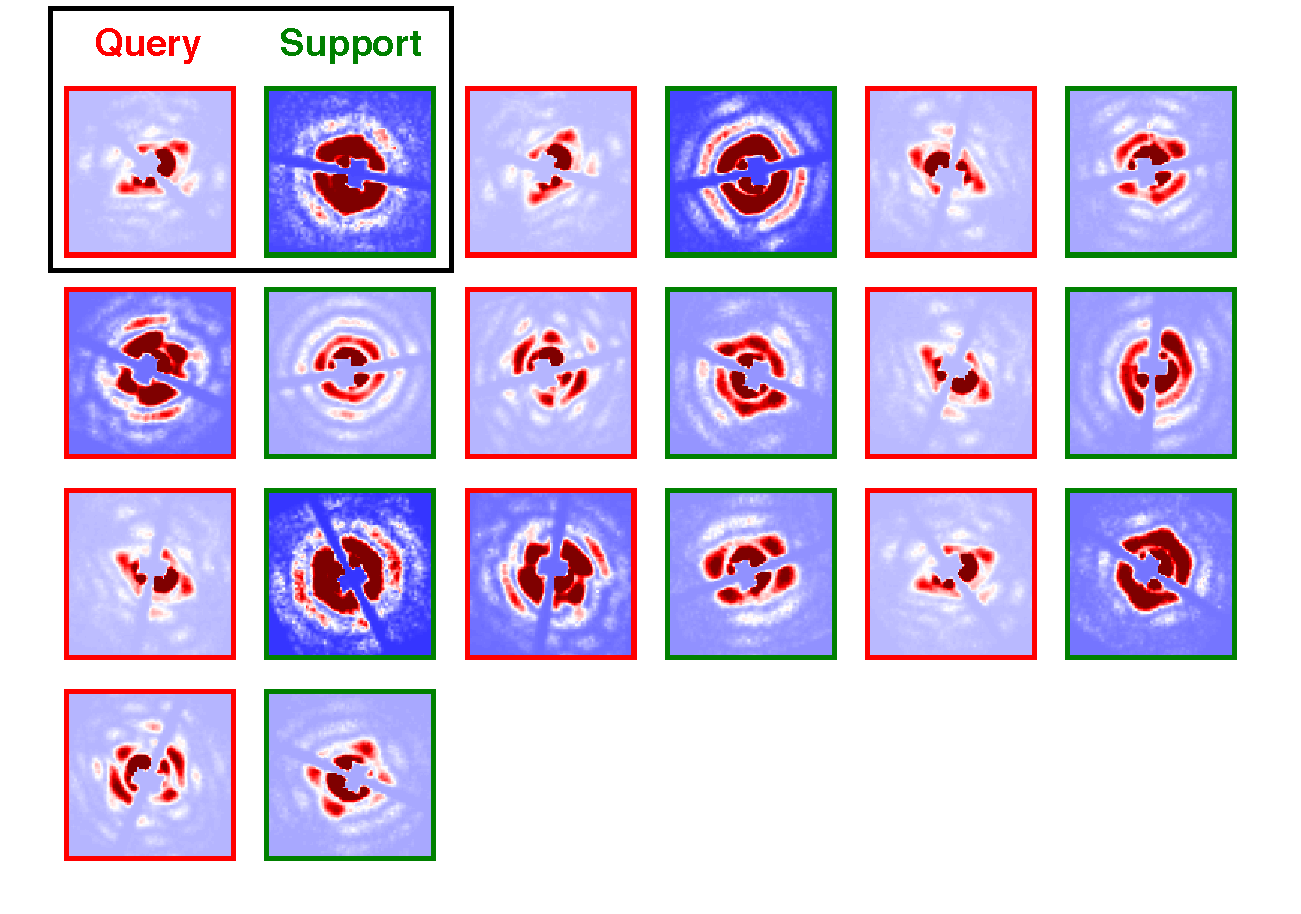
\includegraphics[width=\textwidth,keepaspectratio]
{figures/false_label.single.real.pdf}

\caption{\textit{All} falsely labeled \textit{single-hit} in experiment 4.
Queried samples are put into red boxes, whereas the corresponding most similar
supported samples chosen by our model are enclosed in green boxes.}

\label{fig : false single real}
\end{figure}


To sum it up, data variety plays a critical role in dictating the model
performance that requires covering enough data space.  From a practical
perspective, a good precision of predicting \textit{single-hit} would suffice
for our use.  However, it is recall that reveals whether the data variety is
sufficient, which is the underlying limiting factor that prevents the model from
achieving a better precision.  Additionally, we can label far fewer \textit{hit}s 
for model training if a higher error rate is acceptable by the downstream
particle reconstruction process.  


\subsubsection{Effects of dead detector areas on model performance}

It's not uncommon to encounter a detector with dead pixel areas during a SPI
experiment.  We trained our model on \textit{hit}s artificially occluded by a
mask half of the size of a detector image.  We reused the experiment dataset
mentioned before.  More specifically, We employed 50\% data for model training
and 25\% data each for validation and testing, respectively.  Apart from image
occlusion, the same data preprocessing procedures used in experiment 2 were also
applied, including image cropping, in-plane random rotation, and downsampling.
Through the random in-plane rotation, we prepared 4,000 samples for model
training.  Our model achieves an impressive 100\% (after rounding) precision in
predicting \textit{single-hit}, as seen in Table \ref{tb : real performance
mask}, even with half of its diffraction pattern occluded.  Fig. \ref{fig : true
single real} shows a collection of queried \textit{hit}s correctly labeled
according to their most similar support \textit{hit}s.  Overall, this result
demonstrates that our model can still have good classification performance in
the presence of dead pixel areas on a detector.  

\begin{table}
    \caption{

        Confusion matrix for the experiment investigating data occlusion on
        model performance.  The acronyms used in this table are consistent with
        the definitions specified in Table \ref{tb : real performance}.

    }

    \label{tb : real performance mask}

        \begin{tabularx}{\linewidth}{ l | X X X X X X X X }
                                  &  N(A) & S(A) & M(A) & ACC(\%)  & PRE(\%)  &
                                  REC(\%)           & SPE(\%)  & F1(\%)   \\
            \hline
            N(P)                  &  331  & 0    &  5   & 99 & 99 & 100 & 99 & 99 \\
            S(P)                  &  0    & 340  &  1   & 99 & \textbf{100} & 99 & 1.00 & 99 \\
            M(P)                  &  0    & 5    & 318  & 99 & 98 & 98 & 99 & 98 \\
        \end{tabularx}
    %% }
\end{table}


\begin{figure}
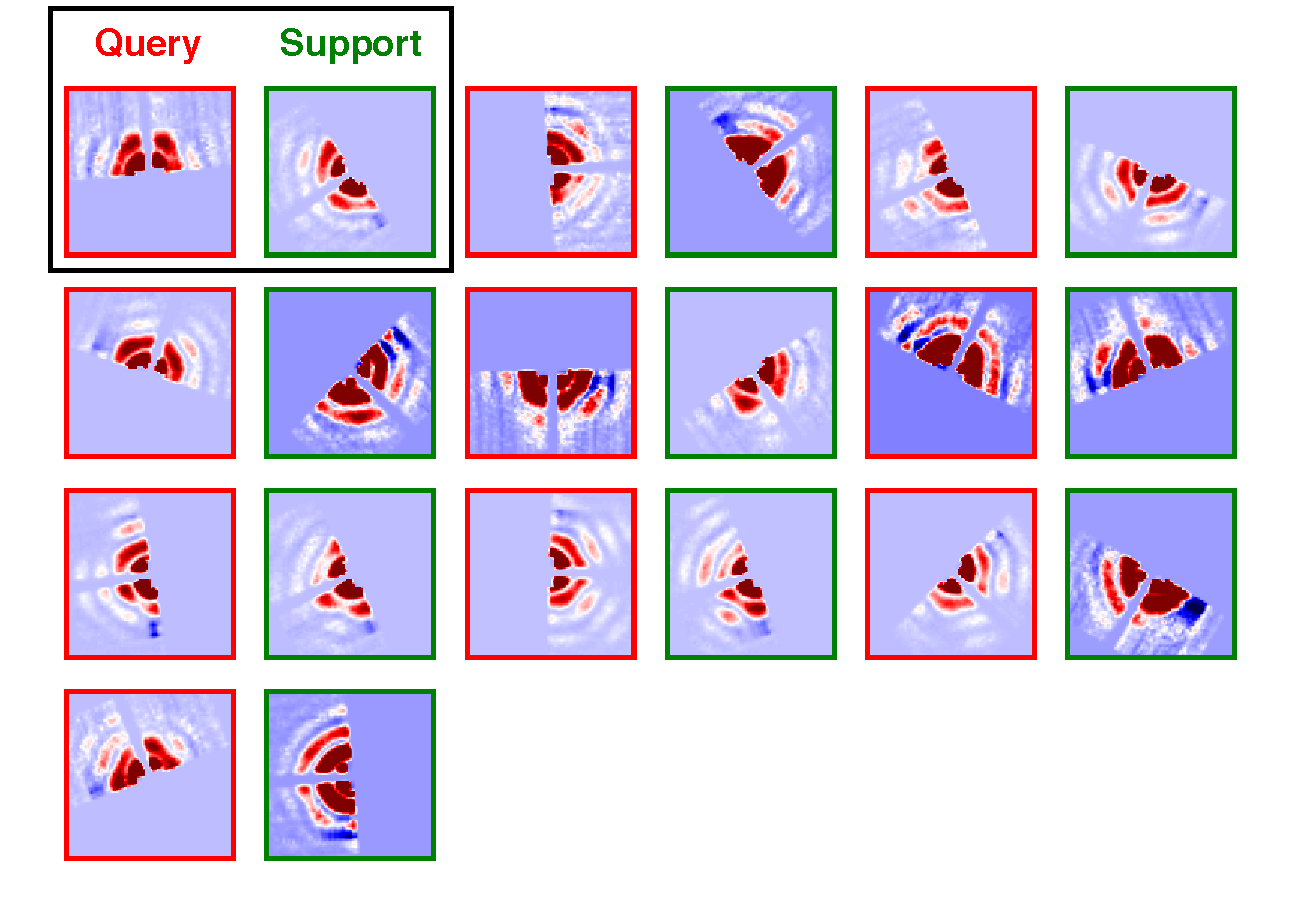
\includegraphics[width=\textwidth,keepaspectratio]
{./figures/true_label.single.real.pdf}

\caption{A partial collection of correctly labeled \textit{single-hit} in the
experiment where SPI hits are artificially occluded to mimic the behavior of a
detector with dead pixel areas.  Queried samples are put into red boxes, whereas
the corresponding most similar supported samples chosen by our model are
enclosed in green boxes.}

\label{fig : true single real}
\end{figure}


\subsection{Model generalizability assessed using simulated hits}

According to the FaceNet paper \cite{schroffFaceNetUnifiedEmbedding2015}, a CNN
vision core trained through a triplet loss function can identify faces of nearly
8 million identities.  It has intrigued us whether our CNN vision core, if
trained in a similar manner, can recognize SPI \textit{hit}s (like human faces)
resulted from various PDB entries (like human identities).  If the
\textit{one-model-fits-all} scenario is true, it will profoundly impact how
\textit{hit} classification can possibly be done in real experiments.  


\subsubsection{Simulated datasets}

There's no existing large scale database of annotated \textit{hit}s generated by
physics-based simulation.  We resorted to \textit{skopi}
\cite{peckSkopiSimulationPackage2022}, a GPU-based program for simulating
diffractive images from noncrystalline biomolecules, for concurrently simulating
high-resolution SPI scattering patterns and providing accurate labels in an
automated manner at scale.  Considering most biological samples in the past SPI
techniques are large virus particles, we are interested in training our
\textit{hit} classifier on \textit{large} single particles.  PDB statistics
offers direct insights into PDB data distribution by molecular weight
(\url{https:
//www.rcsb.org/stats/distribution-molecular-weight-structure}).  Accordingly, we
focus on those particles with molecular weights over 380 $KDa$.  Fig.  \ref{fig:
num atom per bio assem} describes the population frequency of the atom number
per biological assembly with each area representing 50 PDB items.  The atom
numbers spread across three orders of magnitudes ($10^4\text{-}10^6$).  96.0\%
of \textit{large} particles have $10^4$ atoms, and only 1.2\% have massive
$10^6$ atom numbers. Simulated datasets are generated by setting the detector
distance at 100.0 $mm$ and photon energy at 1.660 $KeV$.  In total, we simulated
0.5 million SPI \textit{hit}s from 5,778 PDB entries, and the type of
\textit{hit} ranges from \textit{single-hit} to \textit{quadruple-hit}.  There's
no example of \textit{non-sample-hit} in the simulated dataset.

We divided PDB entries into a training group and a testing group.  Our model had
access to the \textit{hit}s simulated only from the training group during model training
and validation.  Then, the trained model were tested against the \textit{hit}s
simulated only from the PDBs in the testing group.  We chose three ways to
divide PDBs , which were 10\%/90\%, 50\%/50\% and 80\%/20\% (\%training/\%testing).  
The common PDBs in the three testing groups contributed to \textit{hit}s for the
ultimate testing, which contained 115,200 \textit{hit}s from 1,154 PDBs.  

\begin{figure}
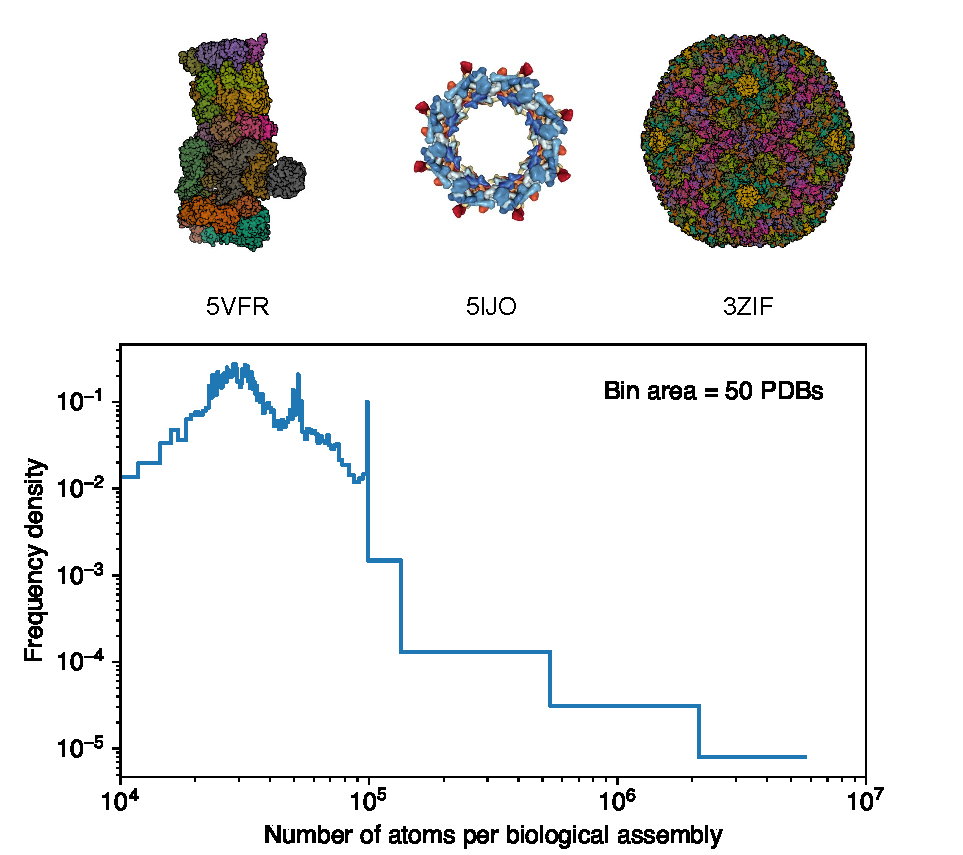
\includegraphics[width=1.0\textwidth,keepaspectratio]
{./figures/num_atom_per_bio_assem.pdf}

\caption{Number of atoms per biological assembly.  Molecular images are taken
from Structure Summary pages from RCSB PDB(rcsb.org) of PDB ID
5VFR\cite{zhuStructuralMechanismNucleotidedriven2018}, 5IJO\cite{kosinskiMolecularArchitectureInner2016} and
3ZIF\cite{chengCryoEMStructuresTwo2014}.}

\label{fig: num atom per bio assem}
\end{figure}


\subsubsection{Performance}

Our model achieved a test accuracy from 90.06\% to 93.38\% on SPI \textit{hit}s
with no noise applied to, which were originally simulated from a diverse
collection of PDB entries.  We investigated four factors that might impact the
model performance.  The primary factor was the noise applied to SPI \textit{hit}
s.  In experiment A1 and A2 in Table \ref{tb : simulated performance}, we kept
\textit{hit}s unperturbed in A1, but applied Poisson noise to \textit{hit}s in
A2 followed by Gaussian noise at the standard deviation of 0.15.  We trained our
model using 200K training examples/\textit{hit}s collected from 80\% PDBs.  The
margin in the triplet loss function was set to be 0.2.  Then, we used 100K
\textit{hit}s in the other 20\% PDBs for testing the model generalizability.
The model in experiment A1 demonstrated an accuracy of 93.38\%, whereas the
noisy \textit{hit}s in A2 reduced the model accuracy down to 86.94\%, a 6.44\%
decline.  The other three factors, which were \%PDB for training, sample size
and triplet loss margin, played a secondary role in dictating the model
performance.  An astonishing finding in experiment B3, C3 and D3
was that our model kept up its accuracy above 90\% even when trained on
\textit{hit}s from only 10\% of PDBs.  Lastly, sample size and triplet loss
margin only turned out to have diminishing effects on improving model
performance.  Fig.  \ref{fig : false single simulated} is an overview of
\textit{all} failed \textit{single-hit} cases in experiment A2.


\begin{table}
    \caption{Experiments that demonstrate the model performances in various
    conditions.}
    \label{tb : simulated performance}
    \begin{tabularx}{\linewidth}{ l | X X X X X }
        Experiment  &
        PDB$_{\text{train}}$ (\%) &
        Sample Size &
        Margin,$\alpha$ &
        Accuracy (\%) \\
        \hline
        A1  & 80 & 200K &  0.2 & 93.38 \\
        A2 (noise)  & 80 & 200K &  0.2 & 86.94 \\
        \hline
        B1  & 80 & 100K &  0.2 & 93.23 \\
        B2  & 50 & 100K &  0.2 & 92.91 \\
        B3  & 10 & 100K &  0.2 & 90.86 \\
        \hline
        C1  & 80 & 100K &  2.0 & 91.56 \\
        C2  & 50 & 100K &  2.0 & 91.00 \\
        C3  & 10 & 100K &  2.0 & 90.84 \\
        \hline
        D1  & 80 & 40K  &  2.0 & 90.20 \\
        D2  & 50 & 40K  &  2.0 & 90.69 \\
        D3  & 10 & 40K  &  2.0 & 90.06 \\
    \end{tabularx}
\end{table}


% Insert the figure HERE and TOP..
\begin{figure}
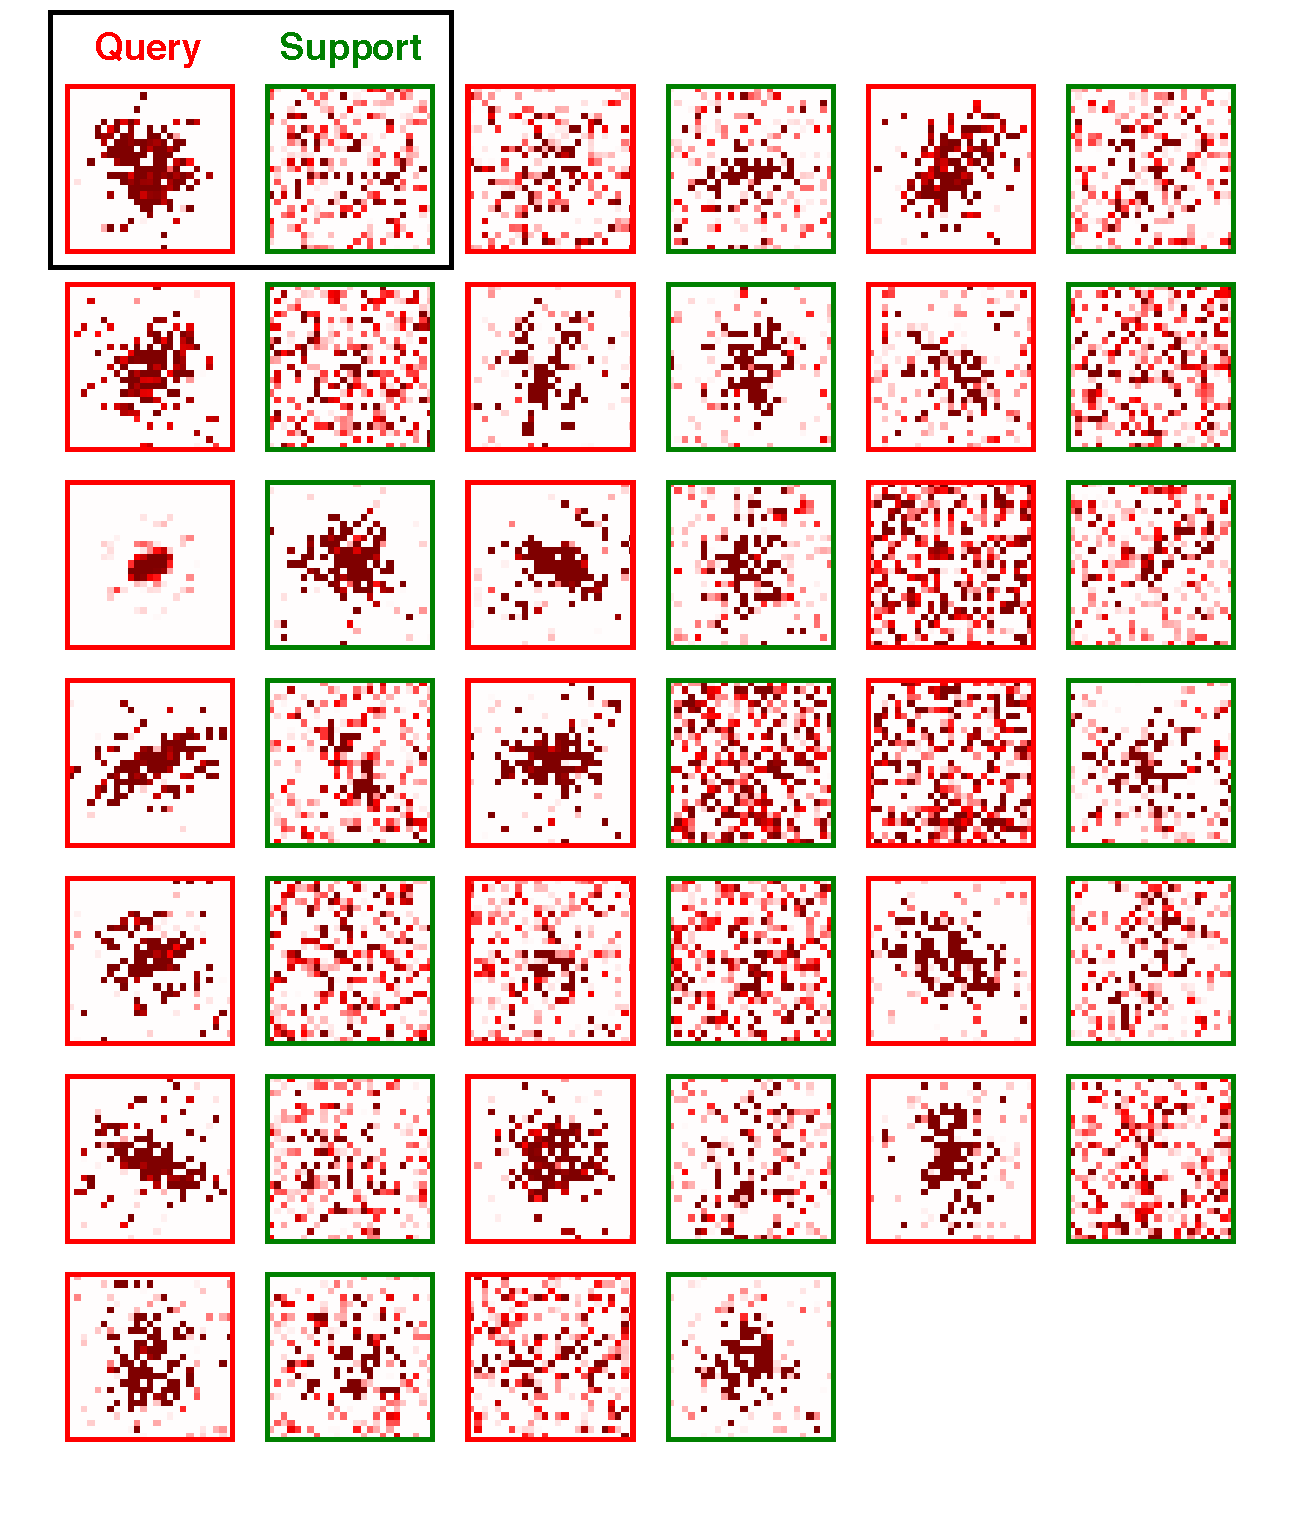
\includegraphics[width=\textwidth,height=0.8\textheight,keepaspectratio]
{figures/false_label.single.simulated.pdf}

\caption{A partial collection of falsely labeled \textit{single-hit} in our test
simulated dataset.  Query samples are put into red boxes, whereas the
corresponding most similar supported samples chosen by our model are enclosed
in green boxes.  The negative intensities are artificially reset to zero for
cleaner visual purposes.  }

\label{fig : false single simulated}
\end{figure}


\subsection{Model performance on simulated PR772 dataset}

We've seen good performance of our model on an experimental PR772 dataset
comprising about 600 manually labeled SPI \textit{hit}s.  Specifically, our
model reached a 99\% precision in predicting \textit{single-hit} by training on
only 80 \textit{single-hit}, 80 \textit{multi-hit} and 44 \textit{non-sample-hit}
.  However, can our model perform consistently well on a larger dataset while
using the same number of training examples?  Complicated by the scarcity of
labeled experimental datasets, we once again turned to \textit{skopi} to
simulate 2,000 \textit{single-hit}, 500 \textit{double-hit}, 300
\textit{triplet-hit} and 200 \textit{quadruple-hit} on an artifical pnCCD
detector with \textit{skopi}.  Like the simulated dataset used in the
generalizability study, there's no \textit{non-sample-hit} class, but we
considered everything other than \textit{single-hit} as \textit{multi-hit}.  

We set aside 50\% of the simulated \textit{hit}s for training but only allowed
80 \textit{hit}s per class visible to our model.  The rest of the dataset were
equally divided by the validation set and the test set.  Afterwards, data
preprocessing was applied in the same manner, which encompassed applying Possion
noise and Gaussian noise, ROI cropping, random in-plane rotation and
downsampling.  In Table \ref{tb : simulated performance large}, the confusion
matrix directly indicates that the model delivers an execellent classification
performance on a larger dataset.  Therefore, we can optimistically conclude that
our model can have a consistently good performance whilst trained on a small
size training set.  

\begin{table}
    \caption{

        Confusion matrix for the experiment investigating model performance on
        a larger dataset.  The acronyms used in this table are consistent with
        the definitions specified in Table \ref{tb : real performance}.

    }

    \label{tb : simulated performance large}

        \begin{tabularx}{\linewidth}{ l | X X X X X X X }
                                  &   S(A) & M(A) & ACC(\%)  & PRE(\%)  & REC(\%)
                                  & SPE(\%)  & F1(\%)   \\
            \hline
            S(P)                  &   477  &  5   & 99 & 99 & 100 & 99 & 99 \\
            M(P)                  &   1    & 517  & 99 & 100 & 99 & 100 & 99 \\
        \end{tabularx}
    %% }
\end{table}


%% Table \ref{tb: SPI
%% experiments} is a list of all SPI experiments documented on CXIDB.  
%% \begin{table}
%%     \caption{All SPI experiments documented on CXIDB.}
%%     \label{tb: SPI experiments}
%%     %% \renewcommand{\arraystretch}{1.2}
%%     %% \resizebox{1.0\textwidth}{!}{
%%         \begin{tabularx}{\textwidth}{ l l X }
%%             CXIDB ID & Light Source & Sample \\
%%             \hline
%%             1        & LCLS         & Mimivirus                                                       \\
%%             2        & LCLS         & Mimivirus                                                       \\
%%             3        & FLASH        & FIB etched 20-nm-thick silicon nitride membrane                 \\
%%             4-8      & ALS          & Gold labeled frozen dried Saccharomyces cerevisiae yeast cells  \\
%%             9        & FLASH        & Iron Oxide Ellipsoids                                           \\
%%             10       & LCLS         & Nanorice                                                        \\
%%             11       & LCLS         & Magnetosomes                                                    \\
%%             12       & LCLS         & Tobacco mosaic virus                                            \\
%%             13       & LCLS         & T4 bacteriophage                                                \\
%%             14       & LCLS         & Paramecium bursaria Chlorella virus                             \\
%%             19       & LCLS         & Airborne Particulate Matter (Soot)                              \\
%%             20       & LCLS         & Clusters of Polystyrene Spheres                                 \\
%%             25       & LCLS         & Carboxysomes                                                    \\
%%             26       & LCLS         & Cyanobium gracile                                               \\
%%             27       & LCLS         & Synechococcus elongatus                                         \\
%%             28       & ALS          & 50 nm colloidal gold particles                                  \\
%%             30       & LCLS         & Mimivirus                                                       \\
%%             36       & LCLS         & Rice Dwarf Virus                                                \\
%%             37       & LCLS         & Cyanobium gracile and Synechococcus elongtatus                  \\
%%             56       & LCLS         & Omono River Virus                                               \\
%%             57       & LCLS         & Gold core and palladium shell nanoparticles                     \\
%%             58       & LCLS         & Coliphage PR772                                                 \\
%%             78       & LCLS         & RNA polymerase II                                               \\
%%             84       & ESRF         & Gold structure (largest diameter about 1.1 um)                  \\
%%             88       & LCLS         & PR772                                                           \\
%%             119      & LCLS         & Sucrose                                                         \\
%%             146      & FLASH        & Xenon nanoclusters                                              \\
%%             155      & LCLS         & Melbournevirus                                                  \\
%%             156      & LCLS         & Coliphage PR772                                                 \\
%%         \end{tabularx}
%%     %% }
%% \end{table}
